Большинство программных систем, имеющих сложную структуру и состоящих из нескольких сотен различных компонент(балансеры, верхние, средние метапоиски, промежуточные и базовые поиски, колдунщики, антироботы, свежесть, региональные поиск, несколько десятков параллельных поисков) обладают рядом схожих проблем. Напимер веб-поиск. Краткое схематичное описание архитектуры:

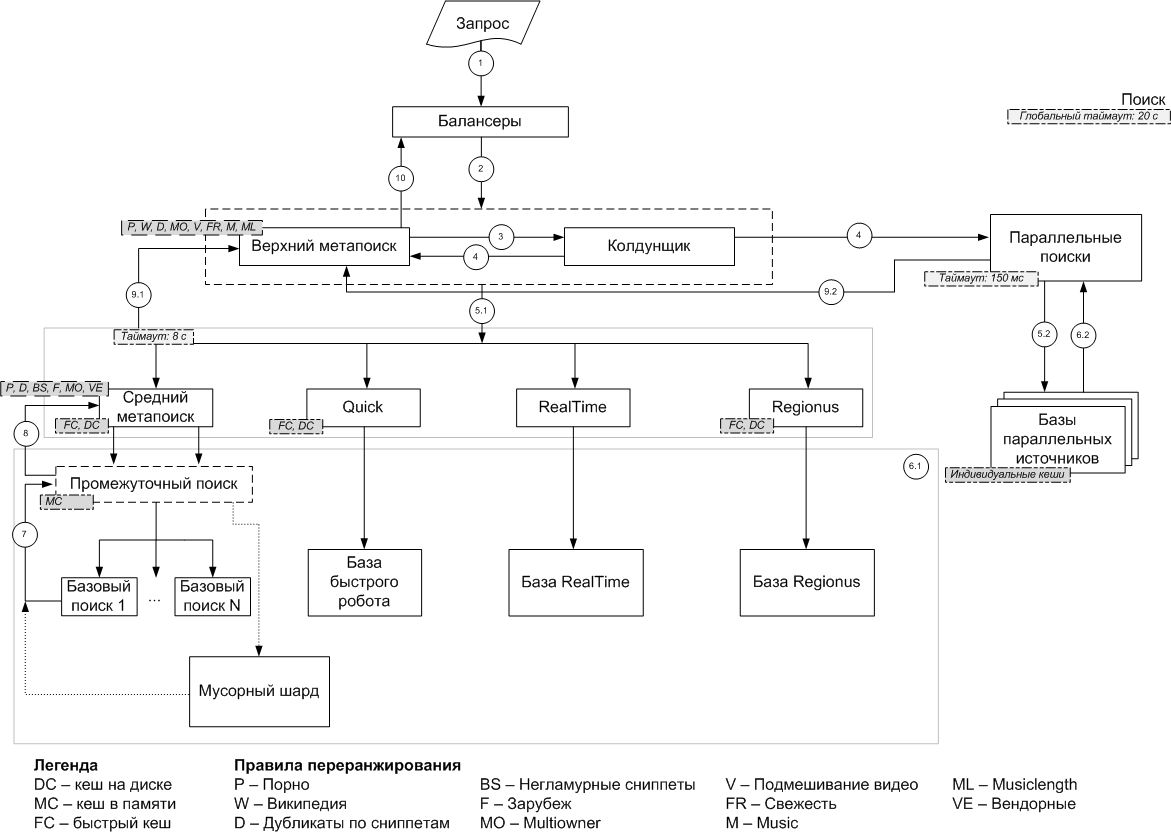
\includegraphics[width=\textwidth]{pics/search.png}

Всего единовременно запущено несколько ******** тысяч приложений. Каждое приложение генерирует множество ошибок и записывает каждую из них в log-файл.
Некоторые приложения, близкие по функционалу, пишут в один и тот же файл. Log-файлы ротируются согласно определённому алгоритму. Тем не менее объем log-файла для одного инстанса приложения может достигать нескольких сотен мегабайт, что препятствует быстрому ручному анализу в случае инцидента и инженеры вынуждены тратить ценные секунды на просмотр сотен тысяч строк файла в поисках сообщения с описанием элемента, вызвавшего сбой работы системы.

Начальным требованием к системе для эффективного использования алгоритма является наличие сопоставимого с количеством поисковых приложений количества нод на которых может быть запущена программа, реализующая алгоритм.

В организации, в которой выполнялась учебно-исследовательская работа, развернута большая поисковая инфраструктура, которая не лишена недостатков и существует вероятность поломки некоторой её части. Существует множество средств мониторинга состояния веб-поиска и противодействия инцидентам, но в некоторых случаях инженерам их недостаточно и приходится вручную анализировать log-файлы отдельных инстансов приложений на отдельных host'ах, что, в свою очередь, замедляет скорость реакции на непредвиденную ситуацию. Но даже автоматизация процесса анализа log-файла на одного инстанса не решает проблему полностью, поэтому необходима возможность быстрого анализа log-файлов сразу множества инстансов.

Таким образом, целью этой учебно-исследовательской работы является разработка алгоритма, позволяющего собирать статистику по ошибкам, встречающимся в log-файлах инстансов поисковых приложений на основе существующих шаблонов и выделять новые шаблоны.
